\documentclass[a4paper, 11pt,oneside]{article}
\usepackage[
  top=1.5cm,
  bottom=1cm,
  left=2cm,
  right=1.5cm,
  headheight=25.22153pt, % as per the warning by fancyhdr
  includehead,includefoot,
  heightrounded, % to avoid spurious underfull messages
]{geometry} 

\usepackage[T1]{fontenc}
\usepackage{microtype}
\usepackage{fancyhdr}
\usepackage{fancyvrb}
\usepackage{lipsum}
\usepackage{url}
\usepackage{listings}
\usepackage{lastpage}
\usepackage{enumitem}
\usepackage{datetime}
\usepackage{amsthm}
\usepackage{graphicx}
\usepackage{hyperref}
\usepackage{minted}
\usepackage{float}

\settimeformat{hhmmsstime}
\yyyymmdddate

\pagestyle{fancy}
\fancyhf{} % clear all fields

\pagestyle{fancy}
\lhead{CMSC 132: Computer Architecture \\ First Semester 2020-2021}
\rhead{Institute of Computer Science \\ University of the Philippines Los Banos}
\rfoot{JACHermocilla (CC NC-BY-SA 4.0)}
%\cfoot{Enjoy!:)}
\cfoot{\thepage\ of \pageref{LastPage}}
\lfoot{Revision: \today\ \currenttime}
%\rfoot{https://jachermocilla.org/teaching/125}
\renewcommand{\headrulewidth}{0.4pt}
\renewcommand{\footrulewidth}{0.4pt}

\begin{document}

\begin{center}
	{\LARGE \textbf{Sequential Logic Circuits}}
\end{center}

\section*{Learning Outcomes}
   At the end of this activity, you should be able to:
   \begin{enumerate}[itemsep=0pt,parsep=0pt]
   	   \item differentiate combinational and sequential elements in a processor;
       \item implement sequential logic circuit elements in VHDL;
   \end{enumerate}   
\tableofcontents

\section{Resources}
\begin{itemize}
	\item Video: \href{https://youtu.be/CzyXb_T-xgU}{https://youtu.be/CzyXb\_T-xgU}.
	\item Source Codes: \href{https://git.io/JU3al}{https://git.io/JU3al}
\end{itemize}	


\section{Discussion}
The discussion in this handout aims only to provide an outline of what is in the video lecture. It is recommended that you watch the video in its entirety.

Sequential elements are sometimes called memory elements because they store state information. The\textit{ output} of any memory element dependes on both the \textit{input} and the \textit{value stored} in it.
An understanding of clocks is important in the study of sequential elements.

\subsection{Clocks}
Clocks determine when the current state of a sequential elements needs to be updated. It is a \textit{signal} that transitions from low to high and high to low in a fixed cycle time or clock period. Figure \ref{fig:clock0} shows an example clock signal. It is a digital signal so it is represented by a square wave and the transition from low to high or high to low is abrupt unline in analog signals. These abrupt transitions are called \textit{clock edges} which may be a \textit{rising edge} (low to high) or \textit{falling edge} (high to low). The \textit{clock period} is the time to complete a cycle and the number of cycles per second is called the \textit{frequency} in \textit{hertz}. The higher the frequency the higher the number of cycles per second. We will use these parameters later when we go to the performance evaluation lab.




\begin{figure}[H]
	\begin{center}
	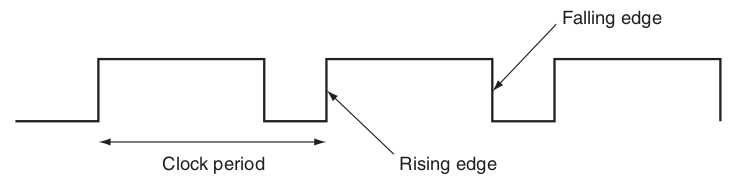
\includegraphics[width=4in]{clock0.png}
	\caption{A clock signal showin the clock period, falling edge, and rising edge.}
	\label{fig:clock0} 
	\end{center}
\end{figure}

The updating of the state element is usually done at the edge of the clock to ensure that the signals will be valid. Figure \ref{fig:clock1} shows a comninational element sandwiched between two state elements. Observe that the updating of the state elements are done at the rising edge. Using the clock edge as marker allows the same state element to be the input and output of the combinational element without invalidating the signal. 

\begin{figure}[H]
	\begin{center}
	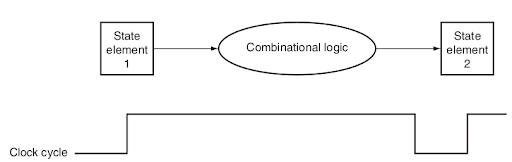
\includegraphics[width=4in]{clock1.png}
	\caption{A combinational element is sandwiched between two state elements. The state elements are updated at the rising clock edge.}
	\label{fig:clock1} 
	\end{center}
\end{figure}


\begin{minted}[frame=single,framesep=10pt]{vhdl}
LIBRARY ieee;
USE ieee.std_logic_1164.all;
ENTITY clocker_tb IS
END clocker_tb;
ARCHITECTURE behavior OF clocker_tb IS
   --100Mhz
   CONSTANT frequency: integer := 100e6; 
   CONSTANT period : time := 1000 ms / frequency;
   SIGNAL clk : std_logic := '0';
BEGIN 
   clk <= not clk after period / 2;
   -- do some stuff here using clk as input
END ARCHITECTURE;
\end{minted}

\subsection{Latches}

\begin{figure}[H]
	\begin{center}
	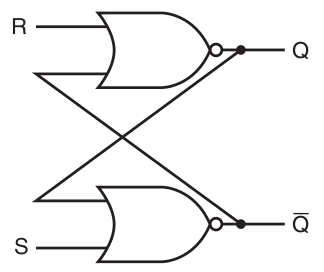
\includegraphics[width=3in]{latch0.png}
	\caption{2-to-1 Multiplexer.}
	\label{fig:mux} 
	\end{center}
\end{figure}

\begin{figure}[H]
	\begin{center}
	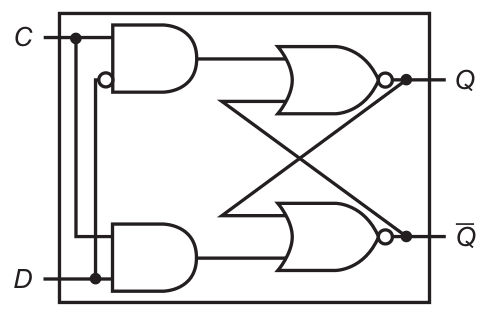
\includegraphics[width=3in]{latch1.png}
	\caption{2-to-1 Multiplexer.}
	\label{fig:mux} 
	\end{center}
\end{figure}

\subsection{Flip-Flops}

\begin{figure}[H]
	\begin{center}
	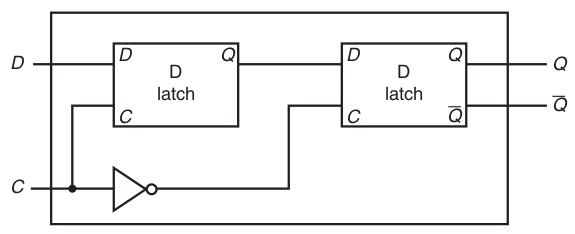
\includegraphics[width=4in]{dff0.png}
	\caption{2-to-1 Multiplexer.}
	\label{fig:mux} 
	\end{center}
\end{figure}

\subsection{Register Files}

\begin{figure}[H]
	\begin{center}
	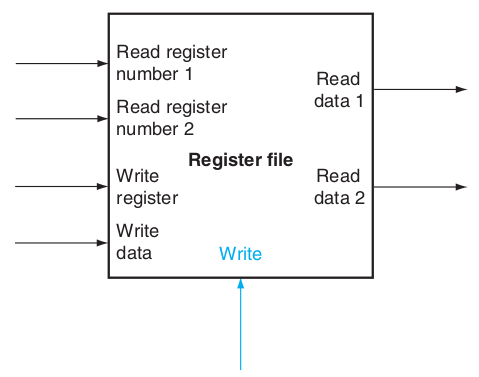
\includegraphics[width=4in]{rf0.png}
	\caption{2-to-1 Multiplexer.}
	\label{fig:mux} 
	\end{center}
\end{figure}

\begin{figure}[H]
	\begin{center}
	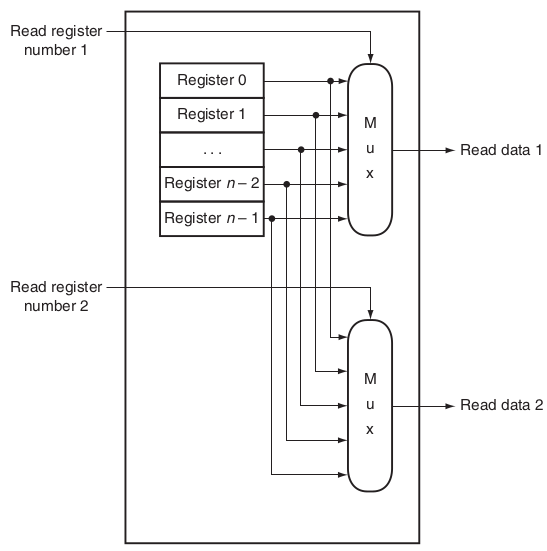
\includegraphics[width=4in]{rf1.png}
	\caption{2-to-1 Multiplexer.}
	\label{fig:mux} 
	\end{center}
\end{figure}

\begin{figure}[H]
	\begin{center}
	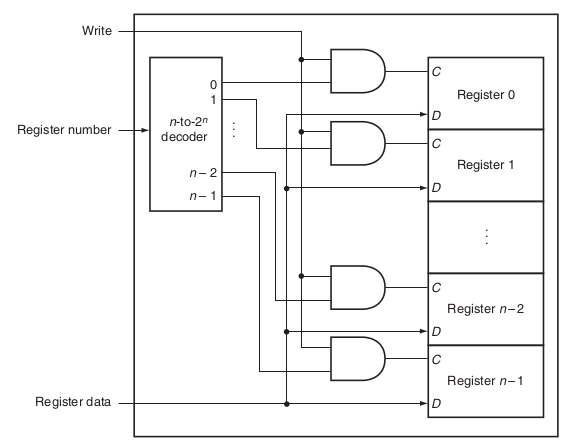
\includegraphics[width=4in]{rf2.png}
	\caption{2-to-1 Multiplexer.}
	\label{fig:mux} 
	\end{center}
\end{figure}

\subsection{Static RAM}

\begin{figure}[H]
	\begin{center}
	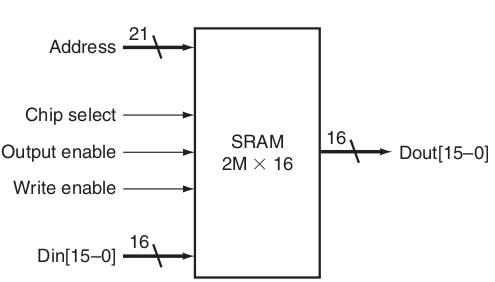
\includegraphics[width=4in]{sram0.png}
	\caption{2-to-1 Multiplexer.}
	\label{fig:mux} 
	\end{center}
\end{figure}

\begin{figure}[H]
	\begin{center}
	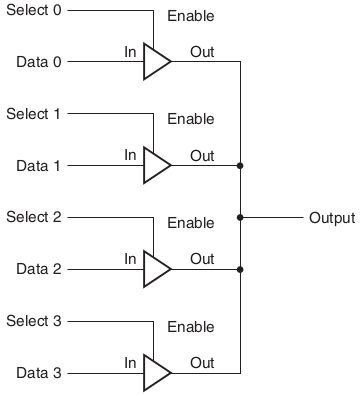
\includegraphics[width=4in]{sram1.png}
	\caption{2-to-1 Multiplexer.}
	\label{fig:mux} 
	\end{center}
\end{figure}

\begin{figure}[H]
	\begin{center}
	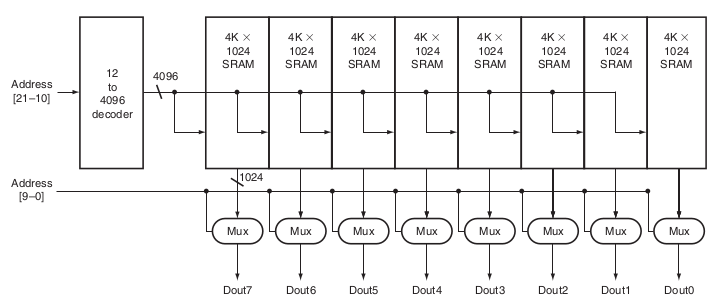
\includegraphics[width=4in]{sram2.png}
	\caption{2-to-1 Multiplexer.}
	\label{fig:mux} 
	\end{center}
\end{figure}



\subsection{Dynamic RAM}

\begin{figure}[H]
	\begin{center}
	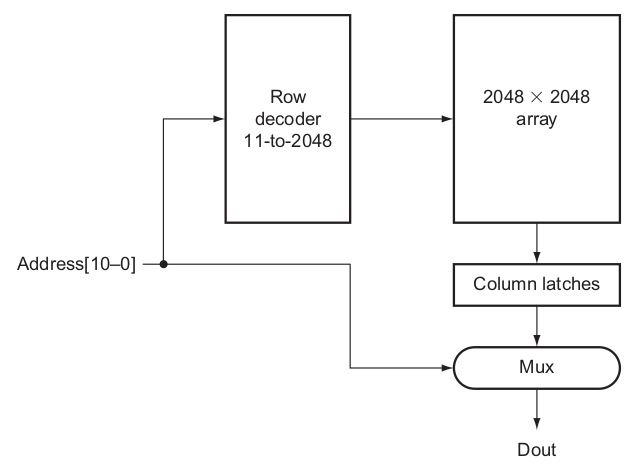
\includegraphics[width=4in]{dram0.png}
	\caption{2-to-1 Multiplexer.}
	\label{fig:mux} 
	\end{center}
\end{figure}


\subsection{Finite State Machines}

\begin{figure}[H]
	\begin{center}
	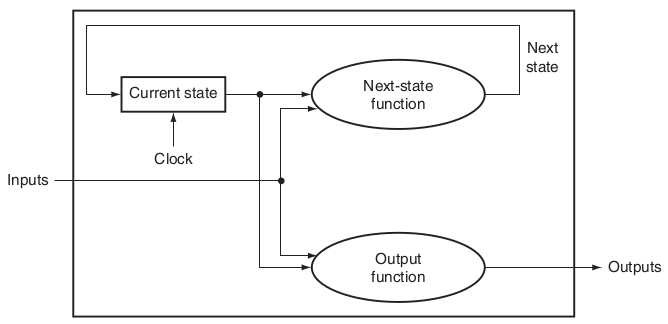
\includegraphics[width=4in]{fsm0.png}
	\caption{2-to-1 Multiplexer.}
	\label{fig:mux} 
	\end{center}
\end{figure}

\begin{figure}[H]
	\begin{center}
	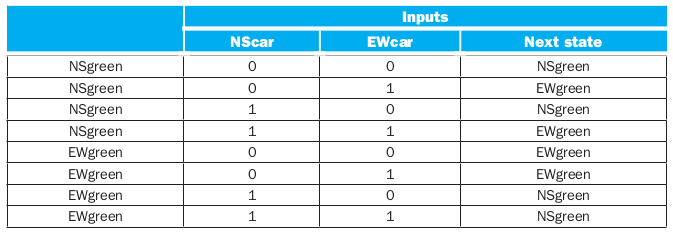
\includegraphics[width=4in]{fsm1.png}
	\caption{2-to-1 Multiplexer.}
	\label{fig:mux} 
	\end{center}
\end{figure}

\begin{figure}[H]
	\begin{center}
	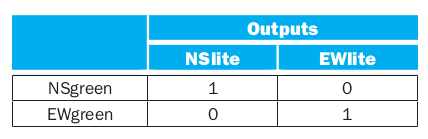
\includegraphics[width=4in]{fsm2.png}
	\caption{2-to-1 Multiplexer.}
	\label{fig:mux} 
	\end{center}
\end{figure}

\begin{figure}[H]
	\begin{center}
	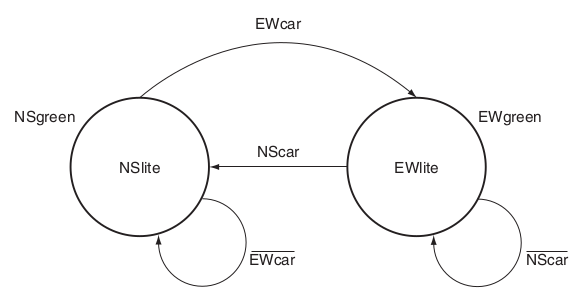
\includegraphics[width=4in]{fsm3.png}
	\caption{2-to-1 Multiplexer.}
	\label{fig:mux} 
	\end{center}
\end{figure}



\begin{minted}[frame=single,framesep=10pt]{vhdl}
LIBRARY ieee;
USE ieee.std_logic_1164.all;
---------------------------------
ENTITY mux_2to1 IS
   PORT (A, B, S: IN STD_LOGIC;
   C: OUT STD_LOGIC);
END mux_2to1;
--------------------------------

ARCHITECTURE pure_logic OF mux_2to1 IS
BEGIN
--- C <= (A AND NOT S) OR (B AND S);                       
   C <= A WHEN S='0' ELSE B;
END pure_logic;
\end{minted}





\section{Summary}
We discussed some of the sequential elements that are useful in the design of a processor. We also showed the design and implementation of a simple traffic light system.

\section{Learning Activities}
Download the source codes for this lab then try experimenting by adding more test cases in the testbenches. Submit a PDF document that shows screenshots of your modifications and runs.

\section{Deliverable}
Your final deliverable for this lab is described in the accompanying exercise handout.

%\begin{thebibliography}{9}
%\end{thebibliography}

\bibliographystyle{unsrt}
\bibliography{seque}
\nocite{*}

\end{document}